\documentclass[margin=10pt]{standalone}
\usepackage{tikz}
\usetikzlibrary{calc}

\begin{document}
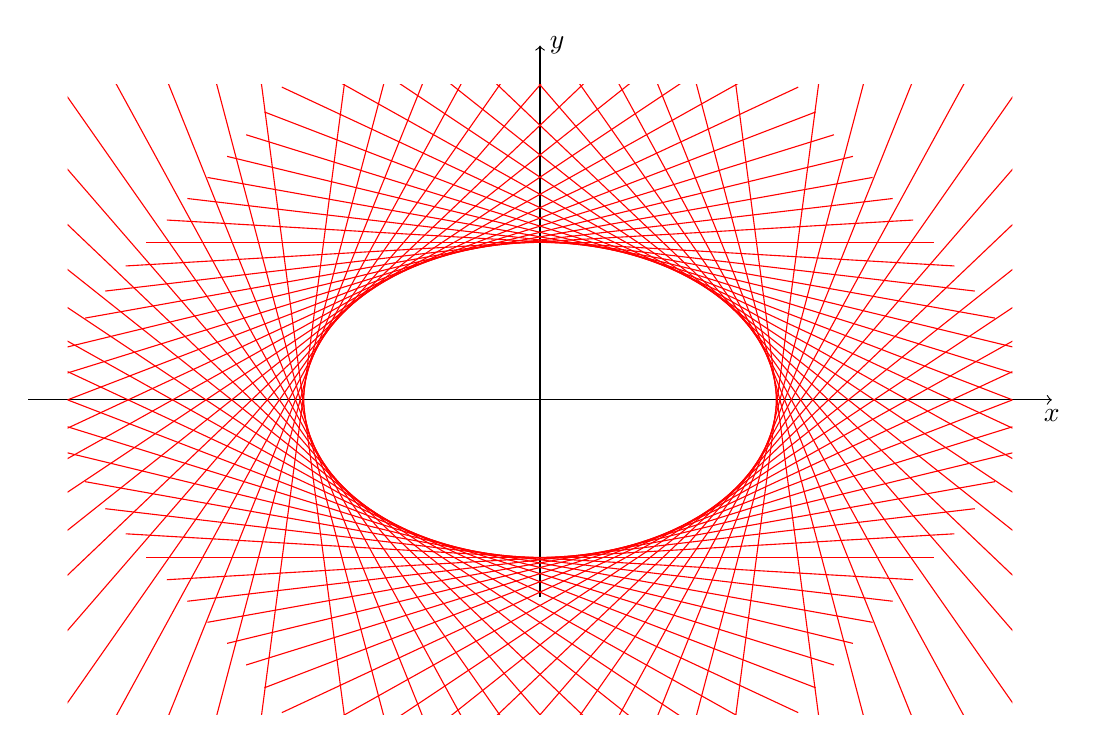
\begin{tikzpicture}

% 画坐标轴
    \draw[->] (-6.5,0) -- (6.5,0) node[below] {$x$};
    \draw[->] (0,-2.5) -- (0,4.5) node[right] {$y$};

    % 画椭圆
    \draw [red](0,0) ellipse (3cm and 2cm);
     \clip (-6,-4) rectangle (6,4);
    % 定义椭圆参数
    \def\a{3}  % 半长轴
    \def\b{2}  % 半短轴
    % 循环绘制切线
    \foreach \theta in {0,5,...,360} {
    \pgfmathparse{\theta} % 设置临时变量
    \let\temp\pgfmathresult % 获取临时变量的值

    % 跳过 0 、180和 360 度
    \ifnum\temp=0
        \pgfmathparse{1} % 设定为 true
        \let\skip\pgfmathresult
    \else
        \ifnum\temp=180
            \pgfmathparse{1} % 设定为 true
            \let\skip\pgfmathresult
    \else
        \ifnum\temp=360
            \pgfmathparse{1} % 设定为 true
            \let\skip\pgfmathresult
        \else
            \pgfmathparse{0} % 设定为 false
            \let\skip\pgfmathresult
        \fi
    \fi
  \fi

    % 如果不是跳过的角度则绘图
    \ifnum\skip=0
        \pgfmathsetmacro\x{\a*cos(\theta)}  % 计算 x 坐标
        \pgfmathsetmacro\y{\b*sin(\theta)}  % 计算 y 坐标

        % 切线方程的斜率
        \pgfmathsetmacro\m{-\b/\a*cot(\theta)}

        % 绘制切线
        \draw[domain=-5:5, red,smooth, variable=\t]
            plot ({\x + \t}, {\m*(\t) + \y});
    \fi
    }
    
\end{tikzpicture}
\end{document}